\clearpage

\section{M-QAM Transmitter}

\begin{tcolorbox}	
	\begin{tabular}{p{2.75cm} p{0.2cm} p{10.5cm}} 	
		\textbf{Header File}   &:& m\_qam\_transmitter.h \\
		\textbf{Source File}   &:& m\_qam\_transmitter.cpp \\
        \textbf{Version}       &:& 20180815 (Manuel Neves)\\
	\end{tabular}
\end{tcolorbox}

This block receives a binary sequence and an optical signal from the local oscillator, with these, it generates a MQAM optical signal. A schematic representation of this block is shown in figure \ref{MQAM_transmitter_block_diagram_simple}.

\begin{figure}[H]
	\centering 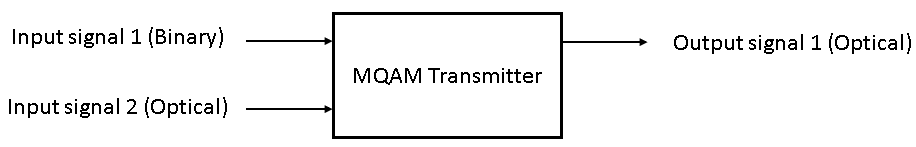
\includegraphics[width=1\textwidth]{./lib/m_qam_transmitter/figures/MQAM_transmitter_block_diagram_simple}
	\caption{Basic configuration of the MQAM transmitter}\label{MQAM_transmitter_block_diagram_simple}
\end{figure}
It also optionally logs in a file the information about the system flow and stores all internal signals for posterior analysis.

\subsection*{Signals}
\begin{subs}
\subsubsection*{Input Signals}
\end{subs}
\hspace*{0.5in}\textbf{Number}: 2\\
\hspace*{0.5in}\textbf{Type}: Binary and Optical
\\
These two input signals are the binary sequence to be transmitted, from the binary source, and the optical signal, directly from the local oscillator of the transmitter.

\begin{subs}
\subsubsection*{Output Signals}
\end{subs}
\hspace*{0.5in}\textbf{Number}: 1\\
\hspace*{0.5in}\textbf{Type}: Optical
\\
The output signal is an optical signal resultant from the modulation of the binary signal at the input with the optical signal from the local oscillator.


\subsection*{Input Parameters}

\begin{table}[H]
\centering
\begin{tabular}{|l|l|l|p{2cm}|}
\hline
\textbf{Name}       & \textbf{Type} & \textbf{Default Value}                & \textbf{Description} \\ \hline
logValue            & bool          & true                                  & If true, the log file will be printed. \\ \hline
logFileName         & string        &  "SuperBlock\_MQamTransmitter.txt"     & Name of the log file. \\ \hline
signalsFolderName   & string        & "signals/SuperBlock\_MQamTransmitter"         & Name of the directory where the internal signals are saved.\\ \hline
\end{tabular}
\caption{Parameters related to the super block}
\end{table}
\begin{table}[H]
\centering
\begin{tabular}{|l|l|p{2.2cm}|p{2.5cm}|}
\hline
\textbf{Name}       & \textbf{Type} & \textbf{Default Value}                & \textbf{Description} \\ \hline
 m & int & 4 & Cardinality.\\ \hline
 iqAmplitudes & vector$<$vector$<$t\_real$>>$ & \{\{1,1\},
  \{-1,1\},
  \{1,-1\},
  \{-1,-1\}\} & Amplitudes of the points of the constellation.\\ \hline
 firstTime & bool & true & First time value on the block M-QAM Mapper. \\ \hline
 numberOfSamplesPerSymbol & int & 8 & Number of samples per symbol.\\ \hline
 impulseResponseTimeLength & int & 16 & Temporal length of the impulse response in multiples of the symbol period. \\ \hline
 filterType & pulse\_shapper\_filter\_type & RaisedCosine & Type of the shaping filter on the pulse shaper block. \\ \hline
 rollOffFactor & double & 0.9 & Roll-off factor for the raised-cosine filter.\\ \hline
 pulseWidth & double & 5e-10 & Width of the pulse.\\ \hline
 passiveFilterMode & bool & false & When true the filter is passive, meaning the amplitudes are normalized.\\ \hline
\end{tabular}
\caption{Configurable parameters related to the blocks inside the MQAM Transmitter}
\end{table}

\subsection*{Block Constructor}

\begin{itemize}
  \item \textbf{MQamTransmitter}(initializer\_list$<$Signal *$>$ inputSig, initializer\_list$<$Signal *$>$ outputSig);
\end{itemize}
This block's constructor expects, as any \textit{Block} object, an input of two vectors of Signal pointers, \textit{InputSig} and \textit{OutputSig}, containing the input/output signals described above.


\subsection*{Methods}
Methods to start and run the block:
\begin{itemize}
     \item void \textbf{initialize}(void);
         \begin{itemize}
             \item[--] Sets up the input and output signals and updates the parameters related to the super block.
         \end{itemize}
     \item bool \textbf{runBlock}(void);
         \begin{itemize}
            \item[--] This method is responsible for iterating over the several blocks contained on the transmitter and running them until the signal buffers are full or all data has been processed.
         \end{itemize}
\end{itemize}
Methods to access/modify system parameters:
\begin{itemize}
     \item void \textbf{setM}(int mValue);
     \item void \textbf{setIqAmplitudes}(vector$<$vector$<$double$>>$ iqAmplitudesValues);
     \item void \textbf{setFirstTime}(bool fTime);
     \item bool \textbf{getFirstTime}(void);
     \item void \textbf{setNumberOfSamplesPerSymbol}(int nSamplesPerSymbol);
     \item int const \textbf{getNumberOfSamplesPerSymbol}(void);
     \item void \textbf{setImpulseResponseTimeLength\_symbolPeriods}(int impResponseTime Length);
     \item int const \textbf{getImpulseResponseTimeLength\_symbolPeriods}(void);
     \item void \textbf{setFilterType}(pulse\_shapper\_filter\_type fType);
     \item pulse\_shapper\_filter\_type const \textbf{getFilterType}(void);
     \item void \textbf{setRollOffFactor}(double rOffFactor);
     \item double const \textbf{getRollOffFactor}(void);
     \item void \textbf{setPulseWidth}(double pWidth);
     \item double const \textbf{getPulseWidth}(void);
     \item void \textbf{setPassiveFilterMode}(bool pFilterMode);
     \item bool const \textbf{getPassiveFilterMode}(void);
\end{itemize}



\subsection*{Examples}
\begin{itemize}
  \item[--] Impact of the constellation coding on the BER:
\end{itemize}
  For this example we will analyse how Grey encoding on the constellation optimizes the BER at the receiver in the presence of noise.
  To achieve that we will use the two following constellations:
    \begin{figure}[H]
    	\centering 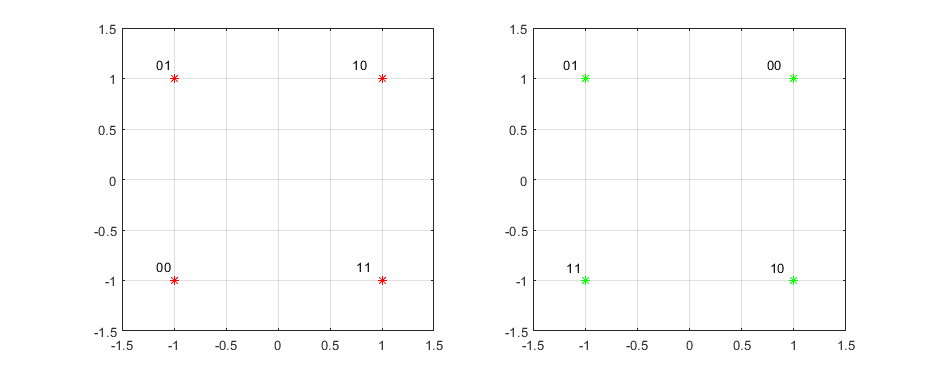
\includegraphics[width=\textwidth]{./lib/m_qam_transmitter/figures/constellations_qpsk.png}
    	\caption{Two different constellations for QPSK.}\label{QPSK_Constellations}
    \end{figure}
  Even though they both seem randomly chosen, after testing these two constellations with all the other parameters constant (the same configuration of the system, apart from the constellation) we get a BER of 10.5\% for the constellation on the left and a BER of 8\% for the constellation on the right.\\
  This happens because, in the presence of noise, the symbols can be decoded to adjacent symbols. And that obviously has an effect on the BER. What we can see here is how the Symbol Error Rate (SER) affects the BER. It's obvious that, once the only configuration that was changed was the constellation, the SER is constant for both cases. \\
  So, what do these two constellations have different to cause different measured BER?\\
  The difference is that, the constellation on the right has Grey encoding, meaning that adjacent symbols only differ in one bit. In this way, a misevaluated symbol will only result in one out of two bits wrong, thus minimizing the BER of a system.
\begin{itemize}
  \item[--] Inter-symbolic interference (ISI) for different pulse shapes:
\end{itemize}
For this example we will analyse the eye diagrams at the receiver side, after the matched receiver filter of the M-QAM Receiver.
\begin{figure}[H]
	\centering
        \begin{subfigure}{.55\textwidth}
        \centering
        	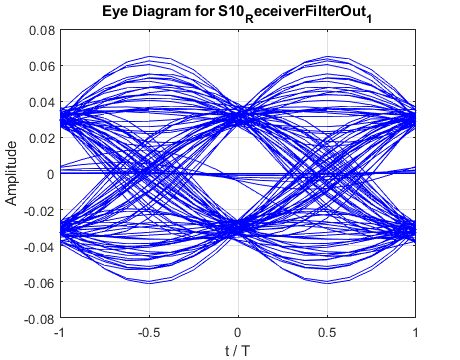
\includegraphics[scale=0.45]{./lib/m_qam_transmitter/figures/eye_dgm_rcos.png}
            \caption{Eye diagram - Raised Cosine}
            \label{r_cos}
        \end{subfigure}%
        \begin{subfigure}{.55\textwidth}
        \centering
        	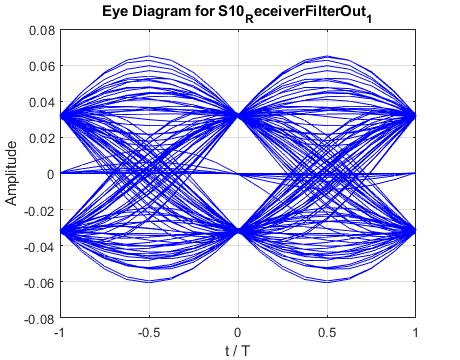
\includegraphics[scale=0.45]{./lib/m_qam_transmitter/figures/eye_dgm_rrcos.png}
        	\caption{Eye diagram - Root Raised Cosine}
            \label{rrcos}
        \end{subfigure}
        \caption{Eye diagrams without noise}%\label{}
\end{figure}
In the figure \ref{r_cos} we have the eye diagram of the received signal, whose pulse was shaped with a Raised Cosine and the matched filter at the receiver had the same filter shape. The result is not what we are expecting, because the Raised Cosine pulse shape is known for having null ISI, but we can clearly see that it is not null. This happens because, thanks to the matched filter, whose shape is the same as the pulse shaper, we actually get a Squared Raised Cosine shape, which does not present the same null ISI as the Raised Cosine impulse.\\
To solve this problem we must instead apply both on the pulse shaper and on the matched filter a Root Raised Cosine filter, in such way that at the receiver we obtain the expected null ISI. The result obtained from this can be observed in figure \ref{rrcos}.\\
Even though that it is clear to see the differences between figures  \ref{r_cos} and  \ref{rrcos}, we have to keep in mind that these signals are ideal and have no noise. It is then of interest to observe if the difference is still noticeable when we have a noise figure with the same order of the ISI seen before.\\
To analyse that we can add noise to the both cases mentioned before, and analyse the differences between both pulse shapes on the eye diagram. The result of doing so can be seen in figures  \ref{noise_r_cos} and  \ref{noise_rrcos}.
\begin{figure}[H]
	\centering
        \begin{subfigure}{.55\textwidth}
        \centering
        	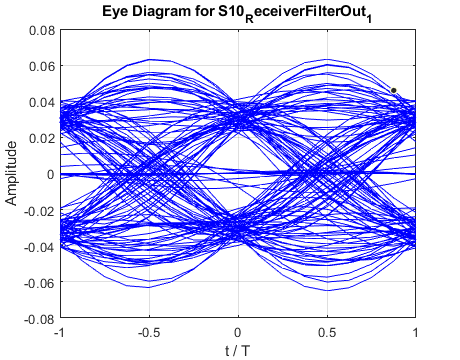
\includegraphics[scale=0.45]{./lib/m_qam_transmitter/figures/eye_dgm_noise_rcos.png}
            \caption{Eye diagram - Raised Cosine with noise}
            \label{noise_rcos}
        \end{subfigure}%
        \begin{subfigure}{.55\textwidth}
        \centering
        	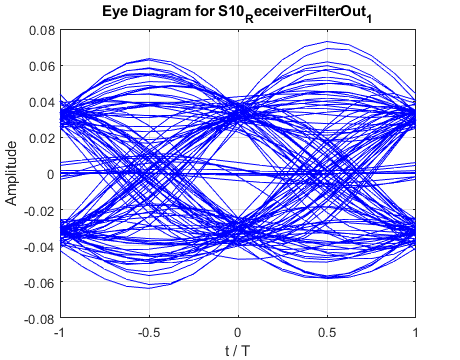
\includegraphics[scale=0.45]{./lib/m_qam_transmitter/figures/eye_dgm_noise_rrcos.png}
        	\caption{Eye diagram - Root Raised Cosine with noise}
            \label{noise_rrcos}
        \end{subfigure}
        \caption{Eye diagrams with noise}%\label{}
\end{figure}
From this we can see that, in spite of one pulse shape having null ISI at the receiver and the other not having, when the noise is of a significant order we can't differentiate both types of pulse shapes as one might expect.


\subsection*{Functional description}

The M-QAM Transmitter is a super block that contains all the necessary blocks to generate a modulated optical signal using only as an input the binary code to modulate and the optical signal from the local oscillator, as we can observe in figure \ref{MQAM_transmitter_block_diagram}.

\begin{figure}[H]
	\centering 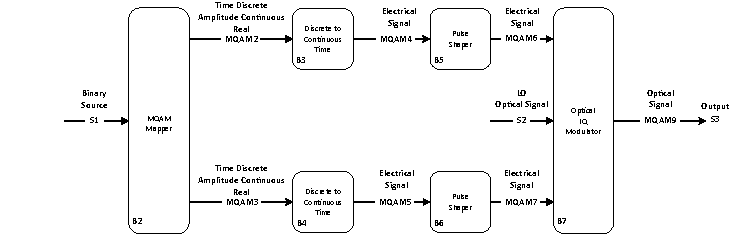
\includegraphics[width=\textwidth]{./lib/m_qam_transmitter/figures/simulation_tx.pdf}
	\caption{Schematic representation of the block MQAM transmitter.}\label{MQAM_transmitter_block_diagram}
\end{figure}
With this block we needn't to manually make all the connections between the different blocks needed to implement an optical transmitter (B1-6). All we need to do is create an instance of the block and only modify the parameters whose default values are not in accordance with our needs. All the methods available to do so have already been presented above.\\
On the next paragraphs, a general overview of the flow of the signal from the input to the output will be made (please note that this is only a simple high-level description, for a detailed analysis of each block you should resort to the respective's block documentation).\\
Firstly, the input signal passes through the M-QAM Mapper, which converts the groups of $\log_2M$ consecutive bits into two streams of \textit{TimeDiscreteAmplitudeContinuousReal} signals (MQAM 1 and 2), these signals have for amplitude the values inserted on the \textit{iqAmplitudes} parameter, in such way that together, they map the binary sequence that originated them.\\
Then, these signals are converted to \textit{TimeContinuousAmplitudeContinuousReal} signals, by up-sampling the previous signals of a factor given by \textit{numberOfSamplesPerSymbol}, obtaining (MQAM 3 and 4).\\
Following, the pulse shaper block uses the previously configured pulse shape (through the input parameters) to turn the pulses into impulses, obtaining signals MQAM 5 and 6, that are the In-phase and Quadrature components used to modulate the optical signal from the input signal 2, henceforth obtaining the output signal 1.\\





\subsection*{Open issues}
\begin{itemize}
  \item[--] the default QPSK constellation isn't the same as the one set if you call the function \textit{setM(4)}, which may originate problems concerning the compatibility with the transmitter;
  \item[--] the block has an unused parameter called \textit{firstTime}, which may cause confusion with the parameter from the M-QAM Mapper, which is accessed and modified through the methods \textit{set/getFirstTime()};
  \item[--] setting a square pulse shape throws a runtime error;
  \item[--] not all methods available at the pulse shaper block can be accessed from the transmitter block.
\end{itemize}
\subsection*{Future improvements}
\begin{itemize}
  \item[--] add missing methods from the pulse shaper to the transmitter block;
  \item[--] add methods to modify the settings of the IQ Modulator;
  \item[--] it would be interesting to have a noise input at the pulse shaper, to be able to see the constellations with noise, because currently there's no easy way to observe this.
\end{itemize}

